%This work is licensed under the Creative Commons License Attribution 4.0 International (CC-BY 4.0)
%https://creativecommons.org/licenses/by/4.0/legalcode
\documentclass[rgb]{standalone}
\usepackage{tkz-euclide}
\definecolor{myorange}{hsb}{0.0833, 1, 0.8}
\definecolor{mygreen}{hsb}{0.3333, 1, 0.8}
\definecolor{myblue}{hsb}{0.5833, 1, 0.8}
\definecolor{mymagenta}{hsb}{0.8333, 1, 0.8}
\begin{document}
	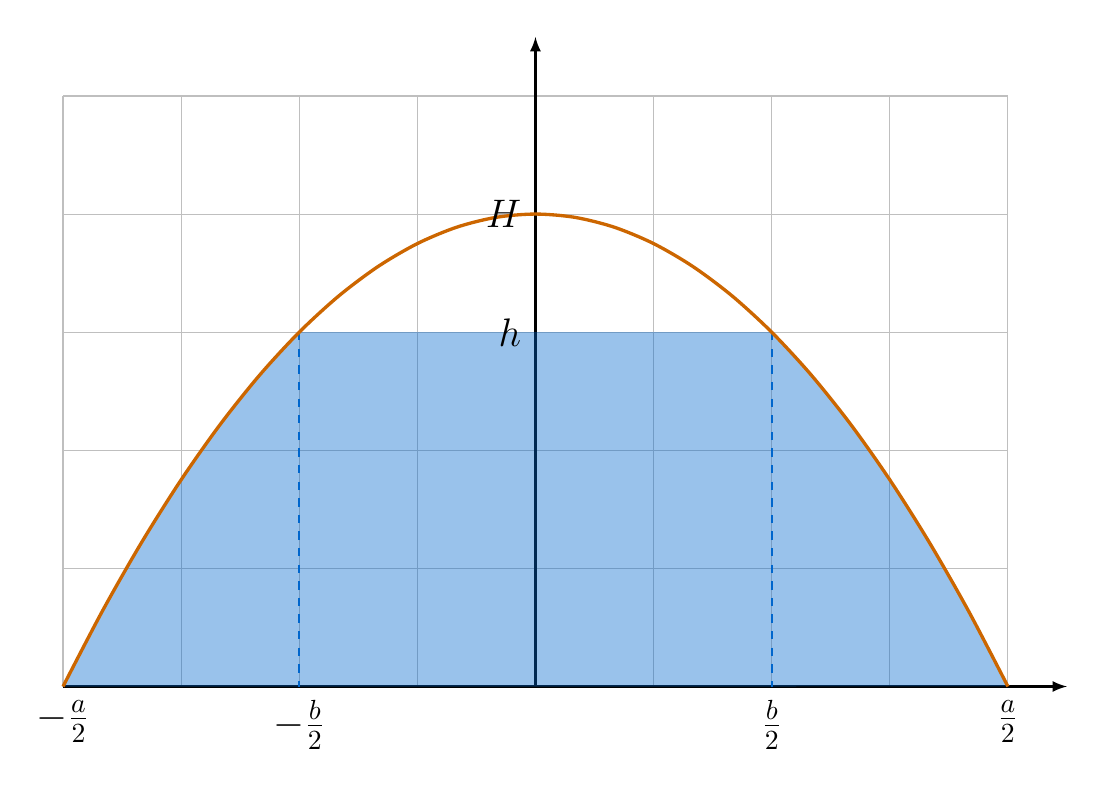
\begin{tikzpicture}[scale=1.5, font=\Large]
		% Coordinate system
		\tkzInit[xmin=-4,xmax=4,ymin=0,ymax=5]
		\tkzGrid[color=lightgray]
	    \tkzDrawX[thick, label=$$]
		\tkzDrawY[thick, label=$$]
	    \draw[fill, draw=none,domain={-4}:{-2}, fill opacity=0.4,smooth,variable=\x,myblue] plot ({\x}, {-1/4*(\x-4)*(\x+4)}) -- (2,3) -- (2,0);
		\draw[fill, draw=none,domain={2}:{4}, fill opacity=0.4,smooth,variable=\x,myblue] (2,0) -- plot ({\x}, {-1/4*(\x-4)*(\x+4)});
		\draw[thick,dashed, myblue] (2,3) -- (2,0);
		\draw[thick,dashed, myblue] (-2,3) -- (-2,0);
		\draw[very thick,myorange,domain={-4}:{4},smooth,variable=\x] plot ({\x}, {-1/4*(\x-4)*(\x+4)});		
		% Labels
        \node[below=0.5mm] at (-4,0){$-\frac{a}{2}$};
		\node[below=0.5mm] at (4,0){$\frac{a}{2}$};
		\node[below=0.5mm] at (-2,0){$-\frac{b}{2}$};
		\node[below=0.5mm] at (2,0){$\frac{b}{2}$};
		\node[left=0.5mm] at (0,3){$h$};
		\node[left=0.5mm] at (0,4){$H$};
	\end{tikzpicture}	
\end{document}